\documentclass[tikz]{standalone}
\usepackage{pgfplots}
\pgfplotsset{compat=1.18}
\begin{document}
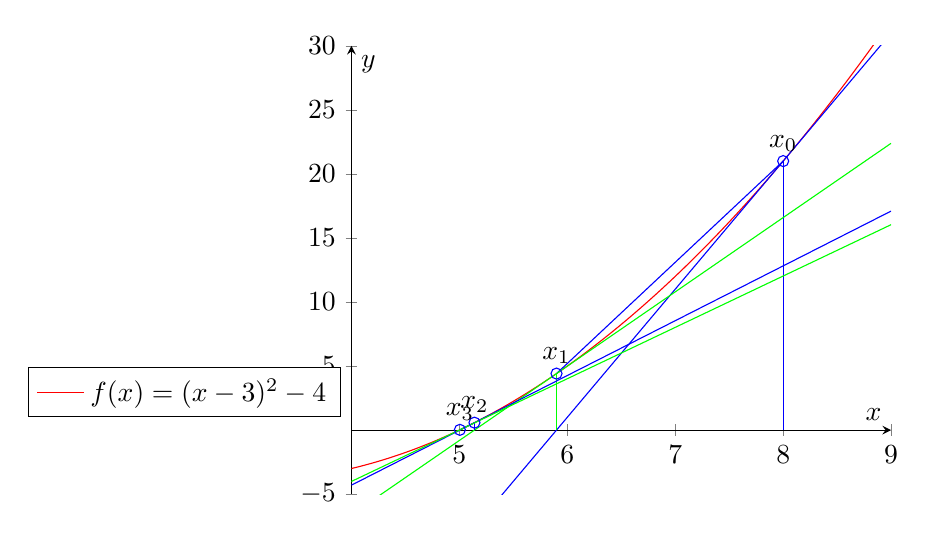
\begin{tikzpicture}
\begin{axis}[
    axis lines=middle,
    xlabel=$x$,
    ylabel=$y$,
    xmin=4,xmax=9,
    ymin=-5,ymax=30,
    xtick={4,...,10},
    ytick={-5,0,5,10,15,20,25,30},
    legend style={at={(axis cs:1,1)},anchor=south west}
]
\addplot[domain=4:9,samples=100,color=red]{(x-3)^2-4};
\addlegendentry{$f(x)=(x-3)^2-4$}
\xdef\xold{8}
\xdef\yold{21}
\foreach \k in {0,...,3}{
    \pgfmathsetmacro{\xnew}{\xold - (pow(\xold-3,2)-4)/(2*(\xold-3))}
    \pgfmathsetmacro{\ynew}{pow(\xnew-3, 2)-4}
    % il punto sulla funzione
    \edef\punto{\noexpand\addplot[
        only marks,
        mark=circle,
        mark size=2pt,
        point meta=explicit symbolic,
        nodes near coords,
        ] coordinates {%
            (\xold,\yold) [$x_{\k}$]%
        };
    }
    \punto
      
    \ifodd\k
        % la tangente
        \addplot[domain=4:9,color=green]{2*(\xold-3)*(x-\xold)+\yold};
        % il segmento verticale
        \addplot[mark=none,color=green] coordinates {(\xold,\yold) (\xold,0)};
    \else
        % il punto sulla funzione
        \addplot[mark=o,color=blue] coordinates {(\xold,\yold) (\xnew,\ynew)};
        % la tangente
        \addplot[domain=4:9,color=blue]{2*(\xold-3)*(x-\xold)+\yold};
        % il segmento verticale
        \addplot[mark=none,color=blue] coordinates {(\xold,\yold) (\xold,0)};
    \fi
%    \addlegendentry{$k=\k$}
    \global\let\xold\xnew
    \global\let\yold\ynew
}
\end{axis}
\end{tikzpicture}
\end{document}